\documentclass{article}
\usepackage[utf8]{inputenc}
\usepackage{listings}
\usepackage{xcolor}
\usepackage{subcaption}
\usepackage{minted}

\definecolor{codegreen}{rgb}{0,0.6,0}
\definecolor{codegray}{rgb}{0.5,0.5,0.5}
\definecolor{codepurple}{rgb}{0.58,0,0.82}
\definecolor{backcolour}{rgb}{0.95,0.95,0.92}
\usepackage{color}   %May be necessary if you want to color links
\usepackage{hyperref}
\usepackage{graphicx}
\hypersetup{
    colorlinks=true, %set true if you want colored links
    linktoc=all,     %set to all if you want both sections and subsections linked
    linkcolor=black,  %choose some color if you want links to stand out
    urlcolor=blue,
}
\lstdefinestyle{mystyle}{
    backgroundcolor=\color{backcolour},   
    commentstyle=\color{codegreen},
    keywordstyle=\color{magenta},
    numberstyle=\tiny\color{codegray},
    stringstyle=\color{codepurple},
    basicstyle=\ttfamily\footnotesize,
    breakatwhitespace=false,         
    breaklines=true,                 
    captionpos=b,                    
    keepspaces=true,                 
    numbers=left,                    
    numbersep=5pt,                  
    showspaces=false,                
    showstringspaces=false,
    showtabs=false,                  
    tabsize=2
}

\lstset{style=mystyle}


\title{SMBUD}
\author{Filippo Lazzati, Martina Magliani, Christian Grasso, Sofia Martellozzo, Giacomo Lombardo}
%\date{October 2021}

\begin{document}
\thispagestyle{empty}
\begin{titlepage}
    \begin{center}
       %\vspace*{2cm}
       {\Huge \textbf{SMBUD}} %%Replace this with the Title of your research
       \vspace{0.5cm}
       \\
    \begin{LARGE}
        {Vaccination and Certificates}
        \vspace{1.0cm}
        \\
        {\textit{Specification, Entity-Relationship model and MongoDB CRUD operations}}
           
\includegraphics[width=13cm]{logo/polimi.png}
          \vspace{1.5cm}\\
                  Filippo Lazzati (10629918) - Martina Magliani (10682333) - Christian Grasso (10652464) - Sofia Martellozzo (10623060) - Giacomo Lombardo (10674987)\\
       {Year: 2021/2022}
    \end{LARGE}  
   \end{center}
\end{titlepage}
\newpage
\tableofcontents %this command creates an index
\newpage
\section{Problem specification}
The purpose of this project is to build an information system that is able to manage pandemic information for a given country. In particular, such system must be scalable enough to manage all the information about COVID-19 tests and vaccinations, and it should provide data at the granularity level required by a business perspective. Moreover, the storage system should be flexible enough in order to comply with the expiration dates of the certificates and, potentially, with the evolution of the rules.\\
Since \verb|MongoDB| is a document-oriented database with the property of being schema-less, it perfectly matches this use case. Furthermore, because of its document-oriented structure, it solves the impedance mismatch problem and, thus, allows to retrieve data also through object-oriented code. The main drawback is the duplication of the data, which is, in a measure, acceptable in the scenario of the certificates.
\section{Hypotheses}
The database is implemented under the following hypotheses:
\begin{itemize}
    \item for each person owning a certificate some demographic details are known;
    \item for each person owning a certificate is also known an emergency contact;
    \item there are 3 different ways through which a person can receive a certificate:
    \begin{enumerate}
        \item healing from the disease; the validity of the certificate is fixed and assumed to be of 6 months after the recovery. A recovery is certified through one negative test after a positive one;
        \item taking at least 1 dose of vaccine; see below for details about the validity of the certificate;
        \item taking a test; the validity varies between the 48 and the 72 hours;
    \end{enumerate}
    \item by definition, a certificate is valid if it contains at least one valid vaccine/test or a certified recovery from the illness;
    \item each person can receive 0, 1 or 2 doses of vaccine (it should be noticed that, up to now, the third dose is not considered; however, since \verb|MongoDB| is schema-less, the introduction of the n-th dose can be easily introduced in the database);
\item there are various types of vaccines, each one of them has different characteristics in terms of validity of the certificate (here, for the sake of simplicity, the vaccines are listed using the name of the brand):
\begin{enumerate}
    \item Pfizer, which provides a valid certificate after 15 days from the first dose and up to 9 months after the administration of the second dose;
    \item Moderna, whose certificates have the same characteristics of the Pfizer's one;
    \item AstraZeneca, whose certificates have the same characteristics of the Pfizer's one;
    \item Johnson \& Johnson, which provides a valid certificate after 15 days from the first dose and valid for 6 months (for the time being we assume this is 
   \item Sputnik, which does not provide any valid certificate because of UE regulations.
\end{enumerate}
It should be noticed that the flexibility offered by a schema-less database like \verb|MongoDB| can be very useful in this case, since the details of the certificates with regards to the type of vaccine can change over time;
\item each vaccine dose is characterized by:
\begin{enumerate}
    \item the name of the brand that produces it;
    \item the name of the vaccine;
    \item the lot of the vaccine;
    \item the production date;
\end{enumerate}
\item a temporary certificate can be obtained also via a COVID-19 test, which can be:
\begin{enumerate}
    \item rapid, which provides a valid certificate for 48 hours;
    \item PCR, which provides a valid certificate for 72 hours;
    \end{enumerate}
\item each test is registered when the result is available and is characterized by the type of the test (rapid/PCR);
\item vaccines and COVID-19 tests can be done in various locations. Each location is characterized by:
\begin{enumerate}
    \item the name of the hospital/health service (or whatever other place like, for instance, a supermarket or the hairdresser) where the vaccine (test) has been administered (performed);
    \item the type of the service (e.g. hospital, local healthcare facility, pharmacy, supermarket etc.);
    \item a full text description of such place;
    \item the address of the location;
    \item the GPS coordinates of the location;
    \item optionally, the department (this can be present only for hospitals and big health structures);
\end{enumerate}
\item the validity of the first dose of vaccine expires 3 months in case the person does not undergoes a second dose;
\item vaccines and tests are administered by authorized health personnel such as doctor and nurses, characterized by name, surname, fiscal code and the position (e.g. nurse, doctor);
\item for each vaccine/test that is administered, the certificate includes the health personnel attending the administration;
\item a doctor/nurse can administer a vaccine in a different place than the workplace (e.g. supermarket or another health structure).
\end{itemize}
\newpage
\section{Conceptual model}
The following is the Entity-Relationship (E-R) model of our database:\\ \\ \\
\vspace{1cm}
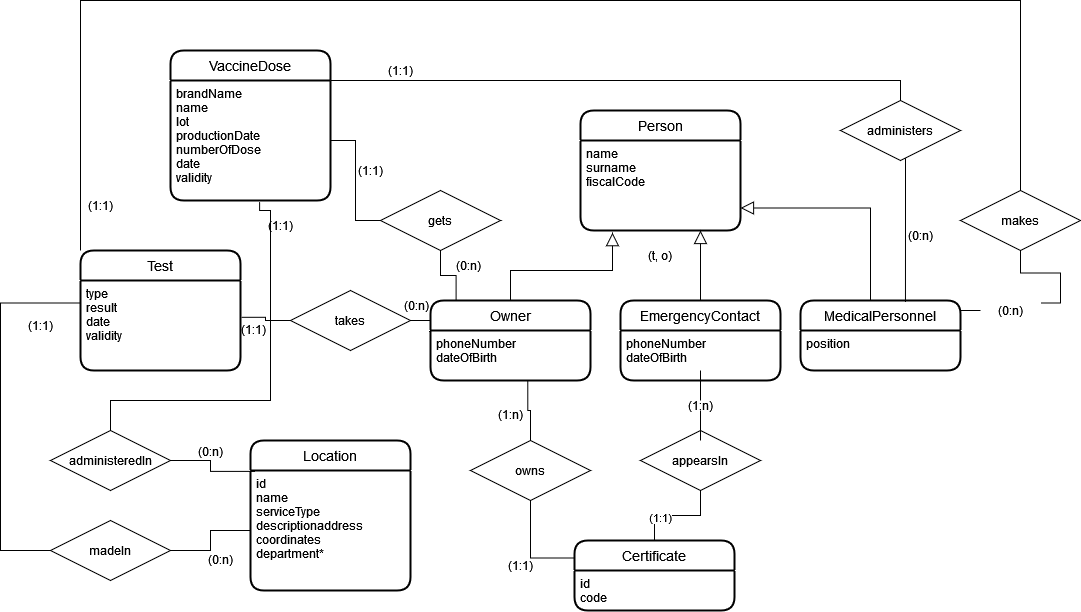
\includegraphics[trim=1cm 1cm 1cm 1cm, width=15cm]{images/e-r.png}
Notice that the optional attributes have been marked with a star (*).\\
The Entity-Relationship model contains 5 main different entities, that are related to each other through various relationships.
\begin{itemize}
    \item \textit{PERSON} represents a person. Every \textit{PERSON} has a name, a surname and a fiscal code. Then there are 3 entities that inherit from \textit{PERSON}, namely \textit{OWNER}, \textit{EMERGENCYCONTACT} and \textit{MEDICALPERSONNEL}. It has been assumed that it is not relevant to insert the date of birth of the \textit{MEDICALPERSONNEL} in the certificate, and that it should be better to avoid to insert its phone number in it. Of course the attributes of \textit{PERSON} could be enlarged, but as a sample dataset we have believed that these three are enough;
    \item \textit{CERTIFICATE} represents the main concept of the whole database. The \textit{CERTIFICATE} will be the document on which we put more or less all the data we have, because the \textit{CERTIFICATE} is at the level of granularity  with which users want to work with this data. We have preferred to represent such entity with only an identifier, since it gains all the data it owns through its relatiosnhips;
    \item \textit{LOCATION} represents a place where a vaccine or a test can be done. It should be remarked that we have decided to detail in-depth such entity, because it is relevant for this scenario. Because of the many attributes it has, you will notice that this is the only document that has not been added to the \textit{CERTIFICATE} document to avoid a useless waste of storage space (as a matter of fact, we have assumed that the \textit{LOCATION} is relevant but it is not required so much from the "business", therefore when it is asked they can wait some additional time);
    \item \textit{VACCINEDOSE} represents one single dose of vaccine received by a person; it has a name, the name of the brand, the lot number and the date of production;
    \item \textit{TEST} represents one single test taken by a person; it is characterised by a type (rapid or PCR), a result, a date and the validity (48 hourse or 72 hours).
\end{itemize}
Among these entities, some relations hold. In particular:
\begin{itemize}
    \item \textit{ADIMINISTERS} and \textit{MAKES} represent the relation between a medical personnel and the vaccine/test he does;
    \item \textit{GETS} and \textit{TAKES} bind a person (\textit{OWNER}) with its doses of vaccine/tests;
    \item \textit{ADMINISTEREDIN} and \textit{MADEIN} specify in which location a certain vaccine dose/test has been administered;
    \item \textit{OWNS} simply relates a person (\textit{OWNER}) to her certificate;
    \item \textit{APPEARSIN} relates the \textit{EMERGENCYCONTACT}s to the certificates in which they appear as such.
\end{itemize}
\newpage
\section{Sample dataset}
The sample dataset we provide is made by the following 2 documents (and all the nested subdocuments). As previously said, the decision of avoid to embed the \verb|LOCATION| documents inside the \verb|CERTIFICATE| ones has been taken in order to prevent a huge and useless waste of storage space. The following is an example of a \verb|CERTIFICATE| document:
\begin{minted}{json}
{
 "_id": "certificate_1",

  "owner": {
    "name": "Mario",
    "surname": "Conte",
    "dateOfBirth": "1978-09-03",
    "fiscalCode": "ZZZ",
    "phoneNumber":"3453298222"
  },

  "emergencyContact": {
    "name": "Mattia",
    "surname": "Calabria",
    "dateOfBirth": "1981-03-11",
    "fiscalCode": "WWW",
    "phoneNumber":"3481222910"
  },

  "vaccineDoses": [
    {
      "type": {
	"brandName": "Pfizer",
        "name": "Comirnaty",
	"lot": "13438242871",
	"productionDate": "2021-05-03"
        },

      "numberOfDose": 1,
      "date": "2021-09-10",
      "location": "locationID",
      "validity": 2160,

      "medicalPersonnel": {
        "name": "Marco",
        "surname": "Inzaghi",
	"fiscalCode": "YYY",
	"position": "doctor"
      }
    }
  ],

  "tests": [
    {
      "type": "rapid",
      "result": false,
      "date": "2021-08-02",
      "location": "locationID",
      "validity": 48,

      "medicalPersonnel": {
        "name": "Matteo",
        "surname": "Rossi",
	"fiscalCode": "XXX",
	"position": "doctor"
      }
    }
  ]
}
\end{minted}
\vspace{0.3cm}
A \verb|CERTIFICATE| document is recognized (like every document in \verb|MongoDB|) by an "\_id" and contains:
\begin{itemize}
    \item the owner of the document;
    \item the emergency contact of the owner of the document;
    \item a list of all the doses of vaccine received (in this way if the rules evolve, additional doses can be added to new documents);
    \item a list of all the tests taken by the owner of the certificate.
\end{itemize}
\vspace{0.3cm}
The \verb|LOCATION| document is the following:
\begin{minted}{json}
{
	"_id": "location_1",
        "name": "Coop",
	"typeOfService": "Supermarket",
	"description": "Coop is a supermarket.",
        "address": "Milano, via Nino Bixio, 64",
        "coordinates": [48, 122]
      }
\end{minted}
It is recognized by an "\_id" and contains all the attributes identified in the conceptual model (E-R) of the data. The \verb|CERTIFICATE| document contains links to it (when needed).\\ \\
\vspace{1cm}
The sample dataset has been created through some \verb|PHP| scripts ..... 
%%%%%%%%%%%%%%%%%%%%%%%%%%%%%%%%%%%%%%%%%%%%%%
chri spiega te
%%%%%%%%%%%%%%%%%%%%%%%%%%%%%%%%%%%%%%%%%%%%%%
\section{Queries and Commands}
The following queries and commands have been developed in order to provide an example of usage of the system for typical usage scenarios.
\subsection{Queries}
We have identified the following different queries:
\begin{enumerate}
    \item \textbf{find all the  valid certificates}.\\ .... Explanation of the query .....
    .....Code of the query ......
    \item \textbf{find the type of vaccine which has been administered the most}.\\ .... Explanation of the query .....
    .....Code of the query ......
    \item \textbf{find the medical personnel who have administered more vaccines}.\\ .... Explanation of the query .....
    .....Code of the query ......
    \item \textbf{find how many vaccinated people there are in the system and how many doses they have done}.\\ .... Explanation of the query .....
    .....Code of the query ......
    \item \textbf{find the people who have taken only tests}.\\ .... Explanation of the query .....
    .....Code of the query ......
    \item \textbf{find the people who have healed}.\\ .... Explanation of the query .....
    .....Code of the query ......
    \item \textbf{find the locations with the highest number of vaccines administered}.\\ .... Explanation of the query .....
    .....Code of the query ......
    \end{enumerate}
\subsection{Commands}
We have identified the following commands to show how the system works:\\
\begin{enumerate}
    \item \textbf{insert a new certificate because of a vaccine dose}.\\ .... Explanation of the command .....
    .....Code of the command ......
    \item \textbf{insert a new certificate because of a test}.\\ .... Explanation of the command .....
    .....Code of the command ......
    \item \textbf{insert a certificate because a new person has received the first vaccine dose}.\\ .... Explanation of the command .....
    .....Code of the command ......
\end{enumerate}
\section{User Interface}
    \subsection{Description}
    We have provided a demo of a User Interface in order to show some use cases of the database and how to apply some sample queries/commands to it. We have implemented a simple client-server application with some basic functionalities to query and update the database. The application is implemented in \verb|JavaScript|, using \textit{node.js} and \textit{express.js} to run the server and the \textbf{React} framework for the front-end.
    \subsection{Functionalities}
    The application allows to:
    \begin{itemize}
    \item ...
    \item ...
    \end{itemize}
\section{User guide}
\subsection{Requirements}
In order to run the application, the following software need to be installed on your machine:
\begin{itemize}
    \item ...
    \item ...
\end{itemize}
\subsection{Database}
To run the database:
\begin{enumerate}
    \item 
\end{enumerate}
\subsection{Server}
After having installed \textit{Node.js}, to run the server do:
\begin{enumerate}
    \item ...
    \item ...
\end{enumerate}
\subsection{Client}
After having started the server, to run the front-end of the application do:
\begin{enumerate}
    \item ...
    \item ...
\end{enumerate}
\section{References and sources}
\begin{itemize}
    \item \href{https://www.mongodb.com}{MongoDB}
    \item \href{https://app.diagrams.net}{draw.io}
    \item \href{https://nodejs.org}{node.js}
    \item \href{https://expressjs.com}{express.js}
    \item \href{https://reactjs.org/}{React}
\end{itemize}
\section{Image gallery}
In this section we include some screenshots showing the appearance of the User Interface (UI). Read the captions for details about what each image represents.
    
\end{document}
